
% ============================================================
% GATE CE2 2025 — Problems and Solutions
% Corrected formatting version
% ============================================================

\small

% ------------------------------------------------------------
% Local spacing
% ------------------------------------------------------------
% A small increase in paragraph spacing and equation-row spacing
% keeps the A5 two-column layout readable without making it loose.
\setlength{\parskip}{0.32cm}
\setlength{\jot}{7pt}

% Small, consistent separation between successive problems/blocks.
\newcommand{\ProblemSpace}{\vspace{0.22cm}}

% ------------------------------------------------------------
% Local formatting helpers
% ------------------------------------------------------------

\newcommand{\CodeRef}[1]{%
    \vspace{0.25em}
    \begin{center}
        \fbox{%
            \begin{minipage}{0.90\columnwidth}
                \centering
                \texttt{#1}
            \end{minipage}%
        }
    \end{center}
}

\newcommand{\Solution}{\par\noindent\textbf{Solution:}\ }

\begin{enumerate}[label=\thesubsection.\arabic*, ref=\thesubsection.\theenumi]




\ProblemSpace
% ============================================================
% Question 3 — Energy consumption
% ============================================================

\item
An electricity utility company charges \rupee 7 per kWh
(kilo watt-hour). If a 40-watt desk light is left on for 10 hours
 each night for 180 days, what would be the cost of energy
consumption? If the desk light is on for 2 more hours each night
for the 180 days, what would be the percentage-increase in the
cost of energy consumption?

\hfill (CE2~2025)

\begin{multicols}{4}\begin{enumerate}[label=\alph*)]
    \item \rupee 604.8; 10\%
    \item \rupee 504; 20\%
    \item \rupee 604.8; 12\%
    \item \rupee 720; 15\%
\end{enumerate}\end{multicols}

\Solution
The initial energy consumption is
\begin{align}
    E_1
    &= P \times t_1 \times N \\
    &= 0.04\,\text{kW}\times10\,\text{hours/night}
       \times180\,\text{days} \\
    &= 72\,\text{kWh}
\end{align}

The initial cost at \rupee 7 per kWh is
\begin{align}
    \text{Initial Cost}
    &= 72\,\text{kWh}\times\text{\rupee }7/\text{kWh} \\
    &= \text{\rupee }504
\end{align}

With $t_2=12$ hours/night, the new energy consumption and cost are
\begin{align}
    E_2
    &= 0.04\,\text{kW}\times12\,\text{hours/night}
       \times180\,\text{days} \\
    &= 86.4\,\text{kWh}, \\
    \text{New Cost}
    &= 86.4\,\text{kWh}\times\text{\rupee }7/\text{kWh} \\
    &= \text{\rupee }604.8
\end{align}

Therefore, the percentage increase is
\begin{align}
    \text{Percentage Increase}
    &= \frac{604.8-504}{504}\times100 \\
    &= 20\%.
\end{align}

Thus, option (B) is correct.

\CodeRef{codes/ce2q3/ce2q3.py}


%% ============================================================
% Question 5 — Ball distribution
% ============================================================

\item
A bag contains Violet ($V$), Yellow ($Y$), Red ($R$), and Green
($G$) balls. On counting them, the following results are obtained:

\begin{enumerate}[label=(\roman*)]
    \item The sum of Yellow balls and twice the number of Violet
          balls is 50.
    \item The sum of Violet and Green balls is 50.
    \item The sum of Yellow and Red balls is 50.
    \item The sum of Violet and twice the number of Red balls is 50.
\end{enumerate}

Which one of the following correctly represents the balls in the bag?

\hfill (CE2~2025)

\begin{enumerate}[label=\alph*)]
    \item $V=10\%$, $R=20\%$, $Y=30\%$, $G=40\%$
    \item $V=40\%$, $R=10\%$, $Y=20\%$, $G=30\%$
    \item $V=30\%$, $R=40\%$, $Y=10\%$, $G=10\%$
    \item $V=20\%$, $R=30\%$, $Y=40\%$, $G=10\%$
\end{enumerate}

\Solution
Let the numbers of Violet, Yellow, Red, and Green balls be represented by
\(V,Y,R,G\), respectively. The four conditions give
\begin{equation}
\vec{A}\vec{x}=\vec{b},
\end{equation}
where
\begin{align}
\vec{x}&=\myvec{V\\Y\\R\\G}, &
\vec{A}&=\myvec{2&1&0&0\\1&0&0&1\\0&1&1&0\\1&0&2&0}, &
\vec{b}&=\myvec{50\\50\\50\\50}.
\end{align}

The augmented matrix is reduced using elementary row operations. The
operations are written directly on the transformation arrows:
\begin{equation}
\resizebox{0.90\linewidth}{!}{$\renewcommand{\arraystretch}{1.12}
\myvec{
2&1&0&0&50\\
1&0&0&1&50\\
0&1&1&0&50\\
1&0&2&0&50
}
\xrightarrow{\;R_1\leftrightarrow R_2\;}
\myvec{
1&0&0&1&50\\
2&1&0&0&50\\
0&1&1&0&50\\
1&0&2&0&50
}
\xrightarrow{\substack{R_2\leftarrow R_2-2R_1\\R_4\leftarrow R_4-R_1}}
\myvec{
1&0&0&1&50\\
0&1&0&-2&-50\\
0&1&1&0&50\\
0&0&2&-1&0
}$}
\end{equation}

Next,
\begin{equation}
\resizebox{0.90\linewidth}{!}{$\renewcommand{\arraystretch}{1.12}
\myvec{
1&0&0&1&50\\
0&1&0&-2&-50\\
0&1&1&0&50\\
0&0&2&-1&0
}
\xrightarrow{\;R_3\leftarrow R_3-R_2\;}
\myvec{
1&0&0&1&50\\
0&1&0&-2&-50\\
0&0&1&2&100\\
0&0&2&-1&0
}
\xrightarrow{\;R_4\leftarrow R_4-2R_3\;}
\myvec{
1&0&0&1&50\\
0&1&0&-2&-50\\
0&0&1&2&100\\
0&0&0&-5&-200
}$}
\end{equation}

Finally,
\begin{equation}
\resizebox{0.60\linewidth}{!}{$\renewcommand{\arraystretch}{1.12}
\myvec{
1&0&0&1&50\\
0&1&0&-2&-50\\
0&0&1&2&100\\
0&0&0&-5&-200
}
\xrightarrow{\substack{R_4\leftarrow-\frac15R_4\\R_1\leftarrow R_1-R_4\\R_2\leftarrow R_2+2R_4\\R_3\leftarrow R_3-2R_4}}
\myvec{
1&0&0&0&10\\
0&1&0&0&30\\
0&0&1&0&20\\
0&0&0&1&40
}$}.
\end{equation}

Hence,
\begin{align}
V&=10, & Y&=30, & R&=20, & G&=40.
\end{align}
The total number of balls is
\begin{align}
T&=V+Y+R+G=100,\\
V&=10\%, & R&=20\%, & Y&=30\%, & G&=40\%.
\end{align}

Hence, option (A) correctly represents the balls in the bag.

\begin{figure}[H]
    \centering
    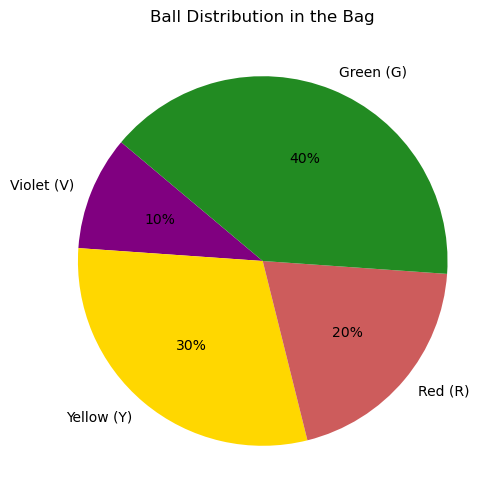
\includegraphics[width=0.5\columnwidth]{figs/piechart.png}
    \caption{Pie chart representing ball distribution.}
    \label{fig:ce2q5_pie}
\end{figure}

\CodeRef{codes/ce2q5/ce2q5.py}



\ProblemSpace
% ============================================================
% Question 8 — Five-digit number
% ============================================================

\item
Consider a five-digit number PQRST that has distinct digits
$P$, $Q$, $R$, $S$, and $T$, and satisfies the following conditions:
$P<Q$, $S>P>T$, and $R<T$. If integers 1 through 5 are used to
construct such a number, the value of $P$ is:

\hfill (CE2~2025)

\begin{multicols}{4}\begin{enumerate}[label=\alph*)]
    \item 1
    \item 2
    \item 3
    \item 4
\end{enumerate}\end{multicols}

\Solution
Combining the inequalities gives
\begin{align}
    R<T<P<Q, \qquad T<P<S.
\end{align}

Since $R<T<P$, the digit $P$ must be greater than at least two
other distinct digits, namely 1 and 2. Hence $P\neq1,2$.

Also, $P<Q$ and $P<S$, so $P$ cannot be the maximum digit 5.
Therefore, the only remaining possibility is $P=3$.

For $P=3$, the smaller digits $\{1,2\}$ can be assigned to
$R$ and $T$, while the larger digits $\{4,5\}$ can be assigned
to $Q$ and $S$. Hence all the inequalities are satisfied.

Thus, option (C) is correct.

\CodeRef{codes/ce2q8/ce2q8.py}


\ProblemSpace
% ============================================================
% Question 9 — Mixture and alligation
% ============================================================

\item
A business person buys potatoes of two different varieties $P$ and
$Q$, mixes them in a certain ratio and sells them at \rupee 192 per kg.
The cost of variety $P$ is \rupee 800 for $5$ kg. The cost of variety
$Q$ is \rupee 800 for $4$ kg. If the person gets $8\%$ profit, what is
the $P:Q$ ratio (by weight)?

\hfill (CE2~2025)

\begin{multicols}{4}\begin{enumerate}[label=\alph*)]
    \item $5:4$
    \item $3:4$
    \item $3:2$
    \item $1:1$
\end{enumerate}\end{multicols}

\Solution
Let the profit percentage be $p=0.08$. Let the cost price of the
mixture be $z$. Since $\text{SP}=z(1+p)$,
\begin{align}
    z&=\frac{192}{1.08}=\frac{1600}{9}\,\text{\rupee/kg},\\
    c_P&=\frac{800}{5}=160\,\text{\rupee/kg}, &
    c_Q&=\frac{800}{4}=200\,\text{\rupee/kg}.
\end{align}

Let $x$ kg of variety $P$ and $y$ kg of variety $Q$ be mixed. Equating
the total cost to the cost of the mixture gives
\begin{align}
    xc_P+yc_Q&=(x+y)z,\\
    x(z-c_P)&=y(c_Q-z),\\
    \frac{x}{y}&=\frac{c_Q-z}{z-c_P}\\
    &=\frac{200-\frac{1600}{9}}{\frac{1600}{9}-160}
     =\frac54.
\end{align}

Thus, the required ratio is $5:4$, making option (A) correct.

\CodeRef{codes/ce2q9/ce2q9.py}


\ProblemSpace
% ============================================================
% Question 10 — Triangle geometry
% ============================================================

\item
Three villages $P$, $Q$, and $R$ are located in such a way that the
distance $PQ=13$ km, $QR=14$ km, and $RP=15$ km. A straight road
joins $Q$ and $R$. It is proposed to connect $P$ to this road $QR$
by constructing another road. What is the minimum possible length
(in km) of this connecting road?

\hfill (CE2~2025)

\begin{multicols}{4}\begin{enumerate}[label=\alph*)]
    \item 10.5
    \item 11.0
    \item 12.0
    \item 12.5
\end{enumerate}\end{multicols}

\Solution
The minimum distance from vertex $P$ to line $QR$ is the altitude
$h_a$. The semi-perimeter of triangle $PQR$ is
\begin{align}
    s=\frac{13+14+15}{2}=21.
\end{align}

Using Heron's formula, the area is
\begin{align}
    \Delta
    &=\sqrt{21(21-14)(21-15)(21-13)} \\
    &=\sqrt{21\times7\times6\times8} \\
    &=84\,\text{km}^2.
\end{align}

Taking $QR=14$ km as the base,
\begin{align}
    h_a=\frac{2\Delta}{14}
       =\frac{2\times84}{14}
       =12\,\text{km}.
\end{align}

Thus, option (C) is correct.

\begin{figure}[H]
    \centering
    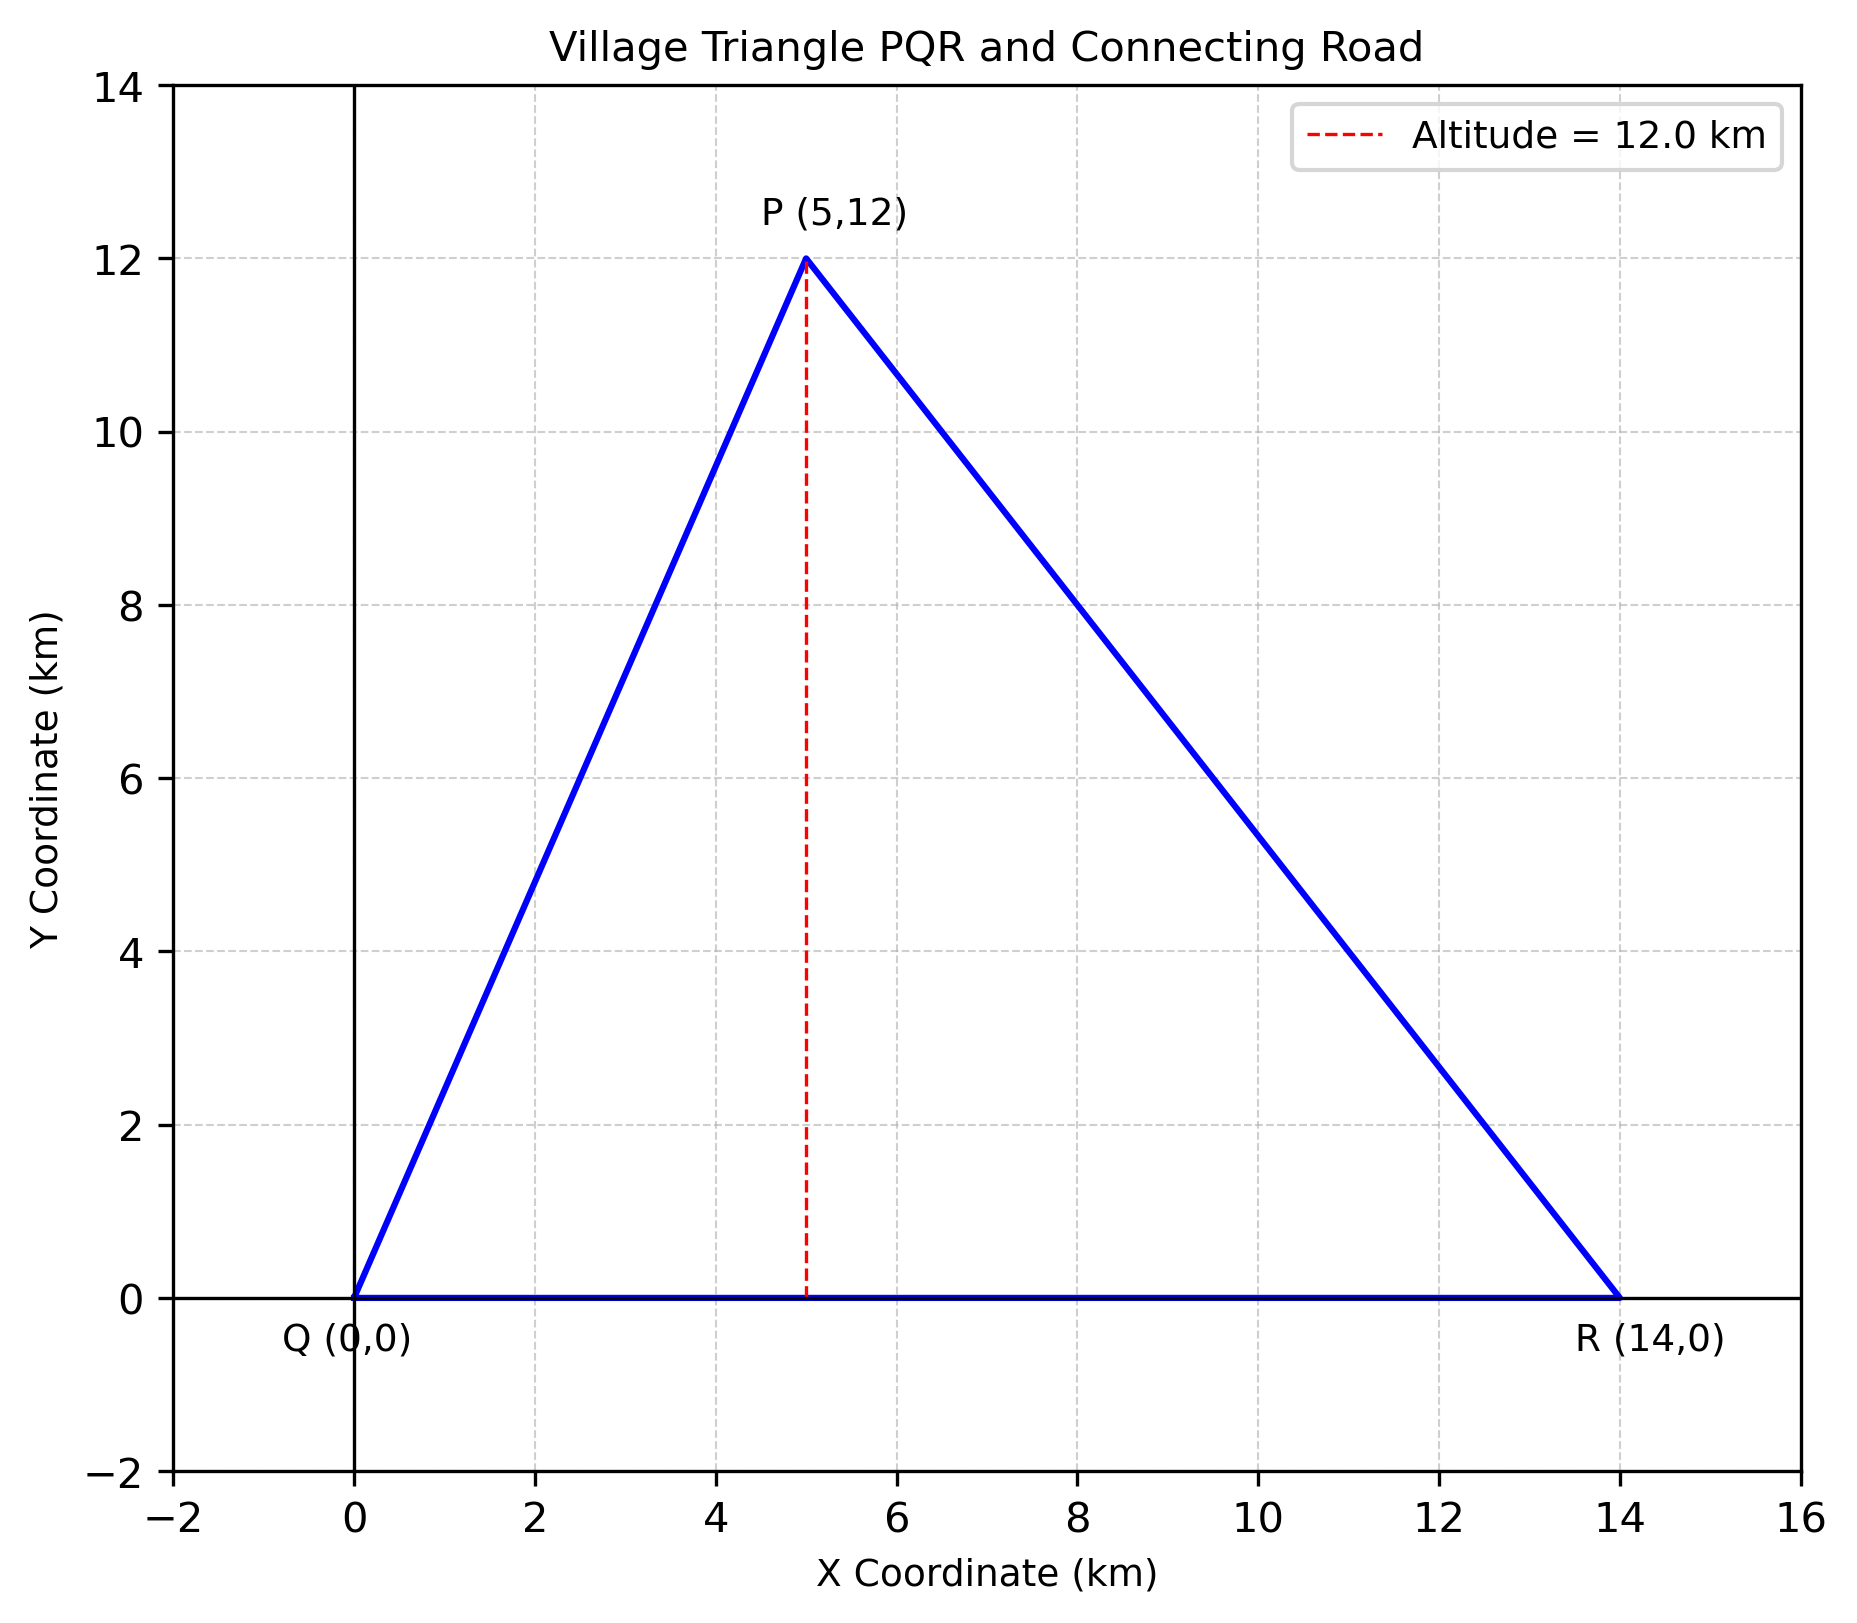
\includegraphics[width=0.8\columnwidth]{figs/village_triangle.png}
    \caption{Triangle $PQR$ geometry and altitude from $P$ to $QR$.}
    \label{fig:ce2q10}
\end{figure}

\CodeRef{codes/ce2q10/ce2q10.py}


\ProblemSpace
% ============================================================
% Question 11 — Matrix transpose
% ============================================================

\item
For the matrix $[\vec{A}]$ given below, the transpose is:
\begin{align}
    [\vec{A}]
    =\myvec{
        2 & 3 & 4 \\
        1 & 4 & 5 \\
        4 & 3 & 2
    }
\end{align}

\hfill (CE2~2025)

\begin{multicols}{4}\begin{enumerate}[label=\alph*)]
    \item $\myvec{2&1&4\\3&4&3\\4&5&2}$
    \item $\myvec{4&3&2\\5&4&1\\2&3&4}$
    \item $\myvec{4&2&3\\5&1&4\\2&4&3}$
    \item $\myvec{2&3&4\\1&4&5\\4&3&2}$
\end{enumerate}\end{multicols}

\Solution
The transpose operation interchanges rows and columns. Therefore,
\begin{align}
    [\vec{A}^{\top}]_{ij}
    &= [\vec{A}]_{ji}, \\
    \vec{A}^{\top}
    &= \myvec{
        2 & 1 & 4 \\
        3 & 4 & 3 \\
        4 & 5 & 2
    }.
\end{align}

Thus, option (A) is correct.

\CodeRef{codes/ce2q11/ce2q11.py}


\ProblemSpace
% ============================================================
% Question 12 — Integration
% ============================================================

\item
Integration of $\ln(x)$ with respect to $x$, i.e.,
$\int\ln(x)\,dx=$\underline{\hspace{3cm}}

\hfill (CE2~2025)

\begin{multicols}{4}\begin{enumerate}[label=\alph*)]
    \item $x\ln(x)-x+C$
    \item $x-\ln(x)+C$
    \item $x\ln(x)+x+C$
    \item $\ln(x)-x+C$
\end{enumerate}\end{multicols}

\Solution
Using integration by parts with $u=\ln(x)$ and $dv=dx$,
\begin{align}
    \int\ln(x)\,dx
    &=x\ln(x)-\int x\cdot\frac1x\,dx \\
    &=x\ln(x)-\int1\,dx \\
    &=x\ln(x)-x+C.
\end{align}

Thus, option (A) is correct.

\CodeRef{codes/ce2q12/ce2q12.py}


\ProblemSpace
% ============================================================
% Question 14 — Influence line of a truss member
% ============================================================

\item
Consider the pin-jointed truss shown in the figure. Influence line
is drawn for the axial force in the member $G-I$, when a unit load
travels on the bottom chord of the truss. Identify the CORRECT
influence line from the options provided, and calculate the axial force values using the section cutting method when the unit load ($1\text{ N}$) is at joints $D$, $G$, $I$, $L$, and $O$.

\hfill (CE2~2025)

\begin{figure}[H]
    \centering
    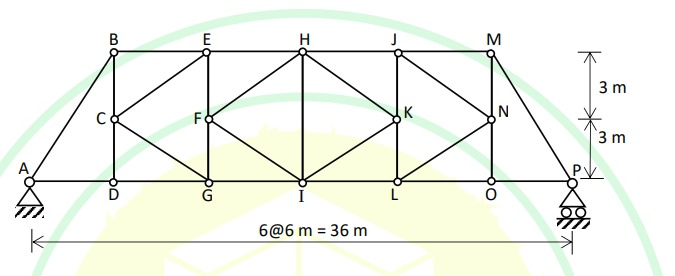
\includegraphics[width=1\columnwidth]{figs/ce2q14.png}
    \caption{Pin-jointed truss for Q14.}
    \label{fig:ce2q14_truss}
\end{figure}

\Solution
An influence line for a truss member shows how the axial force in that
member changes as a unit load moves from one joint to another. Since the
truss is pin-jointed, the moving load is considered only at the bottom
joints \(A, D, G, I, L, O,\) and \(P\), and the variation between joints
is linear.

\subsubsection*{Section Cutting Method and Ordinate Calculations}
To determine the axial force in bottom chord member \(G-I\) using the section cutting method, we pass a vertical section through the panel containing \(G-I\). By considering the equilibrium of the detached portion and taking moments about the corresponding center of moments (the opposite joint), we evaluate the influence coefficients for a unit load ($1\text{ N}$) placed at each bottom chord joint:

\begin{itemize}
\item \textbf{Load at Supports $A$ and $P$:} 
When the unit load is at the end supports, the reactions cause zero internal force in the panel:
\begin{align}
F_{GI}^{(A)} = 0, \quad F_{GI}^{(P)} = 0
\end{align}

\item \textbf{Load at Joint $D$:} 
Cutting the section through the panel and taking moments about the center of moments gives:
\begin{align}
F_{GI}^{(D)} \approx 0.33 \text{ (Tension)}
\end{align}

\item \textbf{Load at Joint $G$ (Panel Point):} 
Using the section method at the panel of member $G-I$, the peak tensile ordinate is obtained as:
\begin{align}
F_{GI}^{(G)} = \frac{4}{3} \approx 1.33 \text{ (Tension)}
\end{align}

\item \textbf{Load at Joint $I$:} 
As the unit load moves to joint $I$, the influence ordinate evaluates to:
\begin{align}
F_{GI}^{(I)} = 1.00 \text{ (Tension)}
\end{align}

\item \textbf{Load at Joint $L$:} 
Similarly, with the load at joint $L$:
\begin{align}
F_{GI}^{(L)} = 0.67 \text{ (Tension)}
\end{align}

\item \textbf{Load at Joint $O$:} 
With the load near the right support:
\begin{align}
F_{GI}^{(O)} = 0.33 \text{ (Tension)}
\end{align}
\end{itemize}

Member \(G-I\) is a bottom chord member. Under a downward moving load,
such members generally develop tensile force, so the influence line is
positive. Among the given options, only option (B) shows a positive piecewise
linear influence line, zero at \(A\) and \(P\), with a maximum ordinate
of \(1.33\) near the panel of member \(G-I\).

Therefore, the correct option is

\begin{equation}
\text{(B)}
\end{equation}

\begin{figure}[H]
    \centering
    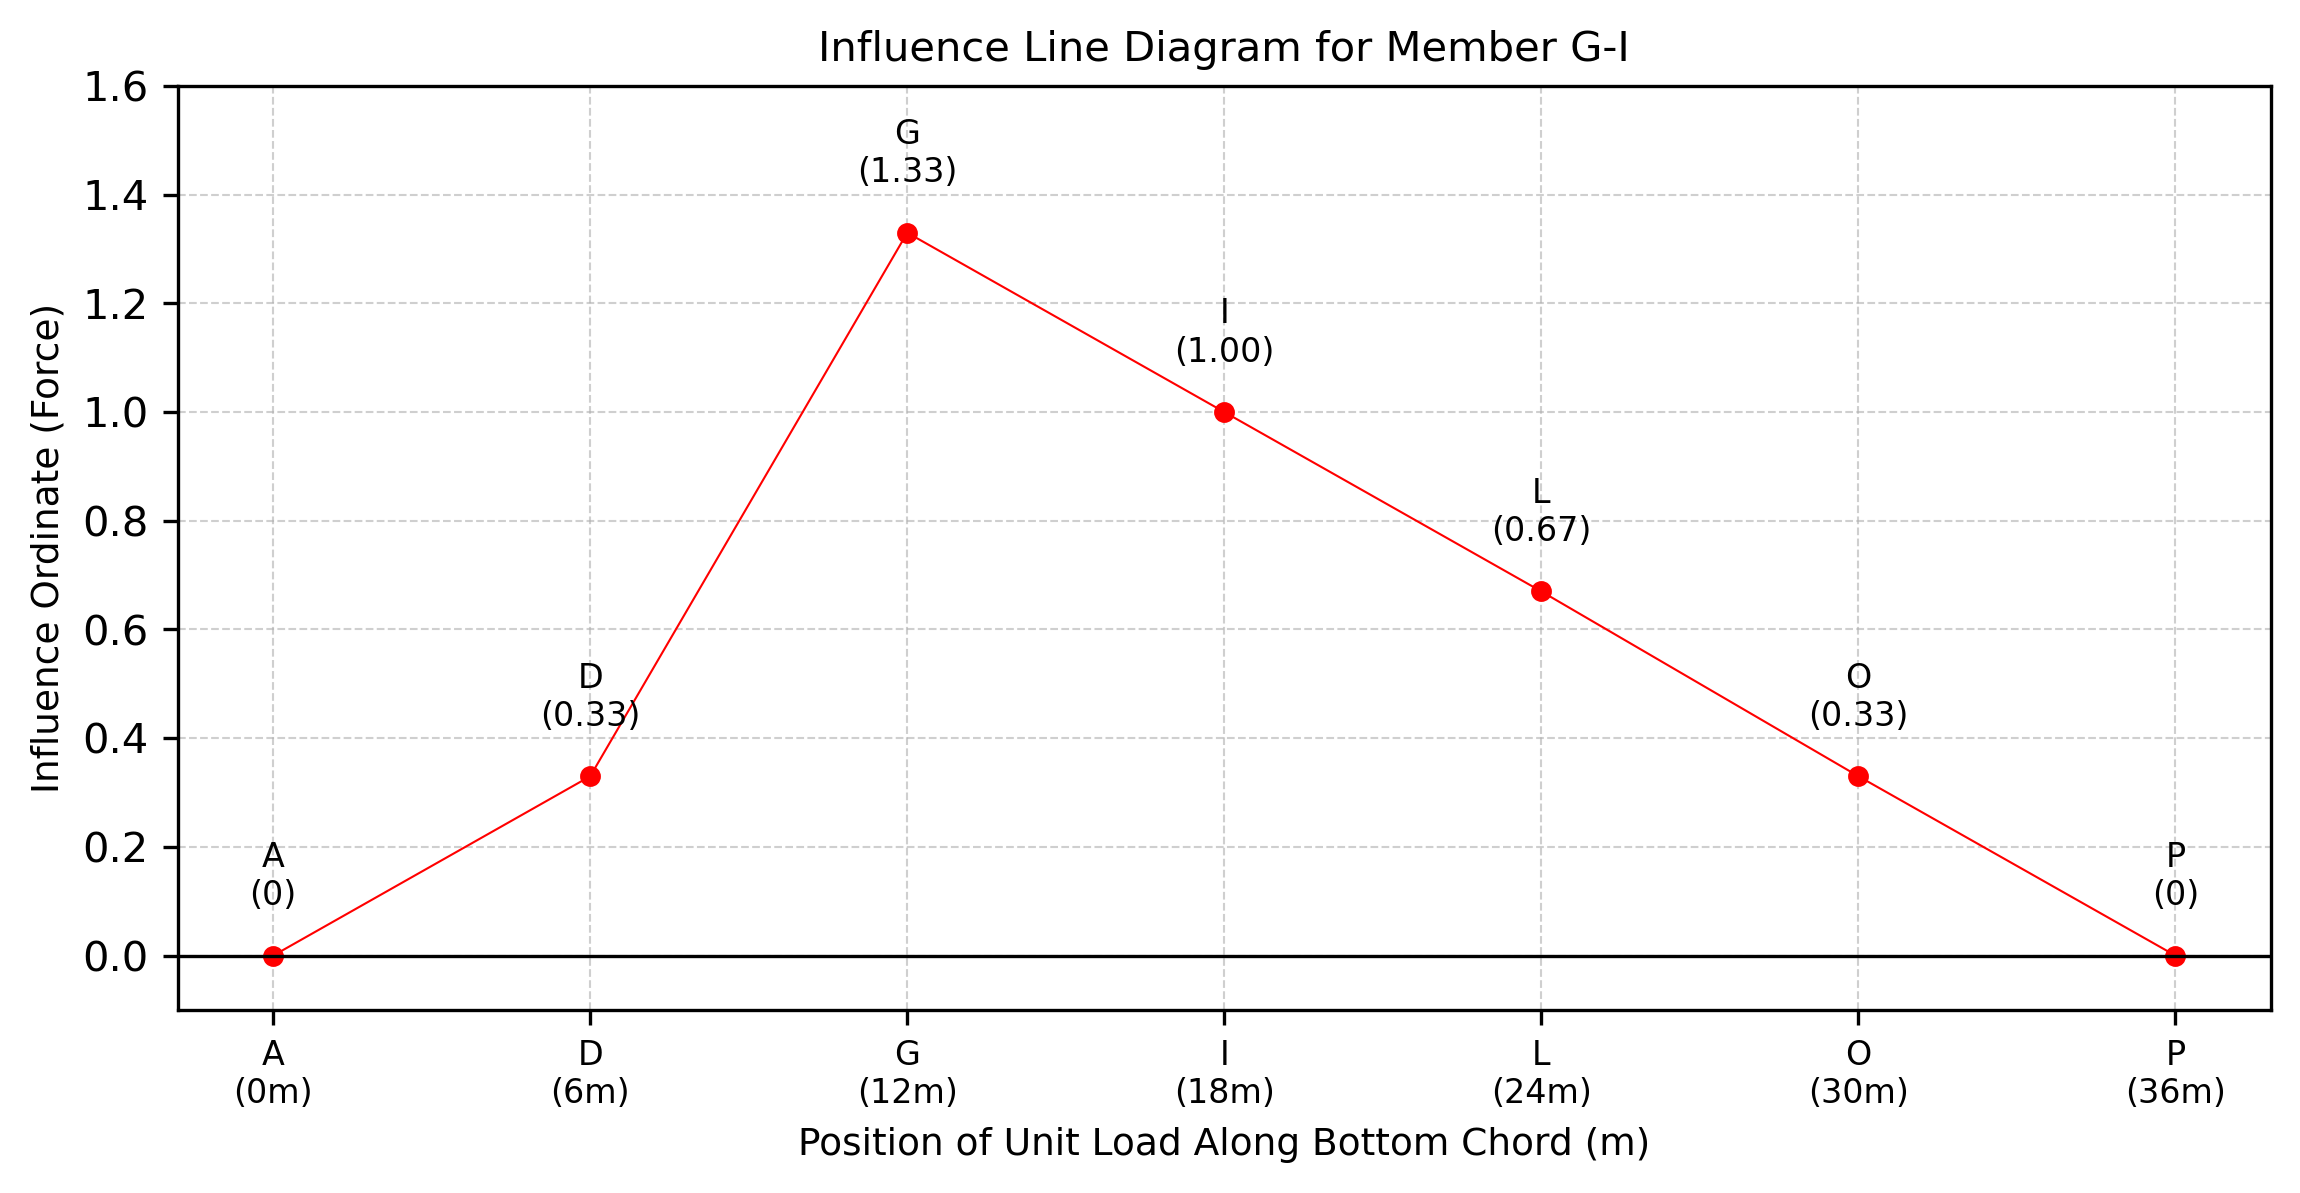
\includegraphics[width=1\columnwidth]{figs/influence_line_gi.png}
    \caption{Correct influence line for axial force in member $G-I$.}
    \label{fig:ce2q14_il}
\end{figure}

\CodeRef{codes/ce2q14/ce2q14.py}


\ProblemSpace
% ============================================================
% Question 21 — Curl and divergence
% ============================================================

\item
Consider a velocity vector $\vec{V}$ in $(x,y,z)$ coordinates given by
$\vec{V}=u\vec{x}+v\vec{y}$. Pick one or more CORRECT statement(s)
from the choices given below.

\hfill (CE2~2025)

\begin{multicols}{2}\begin{enumerate}[label=\alph*)]
    \item $z$-component of Curl of velocity:
          $\nabla\times\vec{V}
          =\left(\frac{\partial v}{\partial x}
          -\frac{\partial u}{\partial y}\right)\vec{z}$
    \item $z$-component of Curl of velocity:
          $\nabla\times\vec{V}
          =\left(\frac{\partial u}{\partial x}
          -\frac{\partial v}{\partial y}\right)\vec{z}$
    \item Divergence of velocity:
          $\nabla\cdot\vec{V}
          =\frac{\partial u}{\partial x}
          +\frac{\partial v}{\partial y}$
    \item Divergence of velocity:
          $\nabla\cdot\vec{V}
          =\frac{\partial u}{\partial y}
          +\frac{\partial v}{\partial x}$
\end{enumerate}\end{multicols}

\Solution
For a two-dimensional velocity field
$\vec{V}=u\vec{x}+v\vec{y}$, the $z$-component of curl is
\begin{align}
    (\nabla\times\vec{V})_z
    =\frac{\partial v}{\partial x}
     -\frac{\partial u}{\partial y}.
\end{align}

Thus, statement (A) is correct.

The divergence is
\begin{align}
    \nabla\cdot\vec{V}
    =\frac{\partial u}{\partial x}
     +\frac{\partial v}{\partial y}.
\end{align}

Thus, statement (C) is correct.

Therefore, the correct statements are (A) and (C).

\CodeRef{codes/ce2q21/ce2q21.py}


\ProblemSpace
% ============================================================
% Question 22 — Probability
% ============================================================

\item
Given that $A$ and $B$ are not null sets, which of the following
statements regarding probability is/are CORRECT?

\hfill (CE2~2025)

\begin{multicols}{2}\begin{enumerate}[label=\alph*)]
    \item $\Pr(A\cap B)=\Pr(A)\Pr(B)$ if $A$ and $B$ are mutually exclusive.
    \item Conditional probability, $\Pr(A\mid B)=1$ if $B\subset A$.
    \item $\Pr(A\cup B)=\Pr(A)+\Pr(B)$, if $A$ and $B$ are mutually exclusive.
    \item $\Pr(A\cap B)=0$, if $A$ and $B$ are independent.
\end{enumerate}\end{multicols}

\Solution
Since $B\subset A$,
\begin{align}
    A\cap B &= B, \\
    \Pr(A\mid B)
    &=\frac{\Pr(A\cap B)}{\Pr(B)}
     =\frac{\Pr(B)}{\Pr(B)}=1.
\end{align}

Hence, statement (B) is correct.

For mutually exclusive events,
\begin{align}
    \Pr(A\cap B)&=0, \\
    \Pr(A\cup B)&=\Pr(A)+\Pr(B).
\end{align}

Hence, statement (C) is correct. Statements (A) and (D) are
incorrect for non-null sets.

Therefore, the correct statements are (B) and (C).

\CodeRef{codes/ce2q22/ce2q22.py}


\ProblemSpace
% ============================================================
% Question 36 — Solution of differential equation using Laplace transform

\item
Pick the CORRECT solution for the following differential equation
\begin{equation}
\frac{dy}{dx}=e^{x-y}.
\end{equation}

\hfill (CE2~2025)

\begin{multicols}{2}
\begin{enumerate}[label=\alph*)]
    \item $y=\ln\brak{e^x+\text{Constant}}$
    \item $\ln(y)=x+\text{Constant}$
    \item $\ln(y)=\ln(e^x)+\text{Constant}$
    \item $y=x+\text{Constant}$
\end{enumerate}
\end{multicols}

\Solution
The nonlinear equation is first transformed using $u=e^y$. 
\begin{align}
\text{Given:}\quad&
\frac{dy}{dx}
&=e^{x-y}=e^xe^{-y},\\[0.04cm]
\text{Let:}\quad&
u
&=e^y,\\[0.04cm]
\text{Then:}\quad&
\frac{du}{dx}
&=e^y\frac{dy}{dx}=e^x,\\[0.04cm]
\text{Laplace transform:}\quad&
\mathcal{L}\left\{\frac{du}{dx}\right\}
&=sU(s)-u(0),\\[0.04cm]
&
\mathcal{L}\{e^x\}
&=\frac{1}{s-1},\\[0.04cm]
\text{Hence:}\quad&
sU(s)-u(0)
&=\frac{1}{s-1},\\[0.04cm]
\text{Therefore:}\quad&
U(s)
&=\frac{1}{s(s-1)}+\frac{u(0)}{s},\\[0.04cm]
\text{Partial fractions:}\quad&
\frac{1}{s(s-1)}
&=-\frac{1}{s}+\frac{1}{s-1},\\[0.04cm]
\text{Thus:}\quad&
U(s)
&=\frac{u(0)-1}{s}+\frac{1}{s-1},\\[0.04cm]
\text{Inverse Laplace transform:}\quad&
u(x)
&=u(0)-1+e^x,\\[0.04cm]
\text{Since }u=e^y:\quad&
e^y
&=e^x+C,\\[0.04cm]
\text{Taking logarithm:}\quad&
y
&=\ln\brak{e^x+C}.
\end{align}

Hence, the correct solution is
\begin{equation}
y=\ln\brak{e^x+\text{Constant}}.
\end{equation}

Therefore, the correct option is (A).

\CodeRef{codes/ce2q36/ce2q36.py}

% ===============================================================
% Question 38 — Propped cantilever with support settlement
% ===============================================================

\item
The figure shows a propped cantilever with uniform flexural rigidity $EI$ (in N.m$^2$)
and subjected to a moment $M$ (in N.m). Consider forces and displacements in the
upward direction as positive.

Find the upward reaction at the propped support $B$ (in N) when this support settles
by $(-\Delta)$, given in metres.

\hfill (CE2~2025)

\begin{multicols}{2}\begin{enumerate}[label=\alph*)]
    \item $\dfrac{3M}{2L}-\dfrac{6EI\Delta}{L^3}$
    \vspace{0.5cm}
    \item $\dfrac{8M}{3L}-\dfrac{2EI\Delta}{L^3}$
    \vspace{0.5cm}
    \item $\dfrac{3M}{2L}-\dfrac{3EI\Delta}{L^3}$
    \vspace{0.5cm}
    \item $\dfrac{M}{L}-\dfrac{8EI\Delta}{L^3}$
    \vspace{0.5cm}
\end{enumerate}
\end{multicols}

\Solution
Treat the reaction at the prop $B$ as the redundant $R_B$. The basic determinate
structure is a cantilever fixed at $A$ and free at $B$. The compatibility and
superposition relations are kept in one aligned block:
\begin{align}
\text{Support settlement:}\quad&
\delta_B
&=-\Delta,\\[0.04cm]
\text{Due to }M:\quad&
\delta_M
&=-\frac{ML^2}{2EI},\\[0.04cm]
\text{Due to }R_B:\quad&
\delta_R
&=\frac{R_BL^3}{3EI},\\[0.04cm]
\text{Compatibility:}\quad&
\delta_M+\delta_R
&=-\Delta,\\[0.04cm]
\text{Hence:}\quad&
-\frac{ML^2}{2EI}+\frac{R_BL^3}{3EI}
&=-\Delta,\\[0.04cm]
\text{Multiplying by }\frac{3EI}{L^3}:\quad&
-\frac{3M}{2L}+R_B
&=-\frac{3EI\Delta}{L^3},\\[0.04cm]
\text{Therefore:}\quad&
R_B
&=\frac{3M}{2L}-\frac{3EI\Delta}{L^3}.
\end{align}

Thus, the upward reaction at support $B$ is
\begin{equation}
R_B=\frac{3M}{2L}-\frac{3EI\Delta}{L^3}.
\end{equation}

Hence, the correct option is (C).

\CodeRef{codes/ce2q38/ce2q38.py}

\begin{figure}[H]
    \centering
    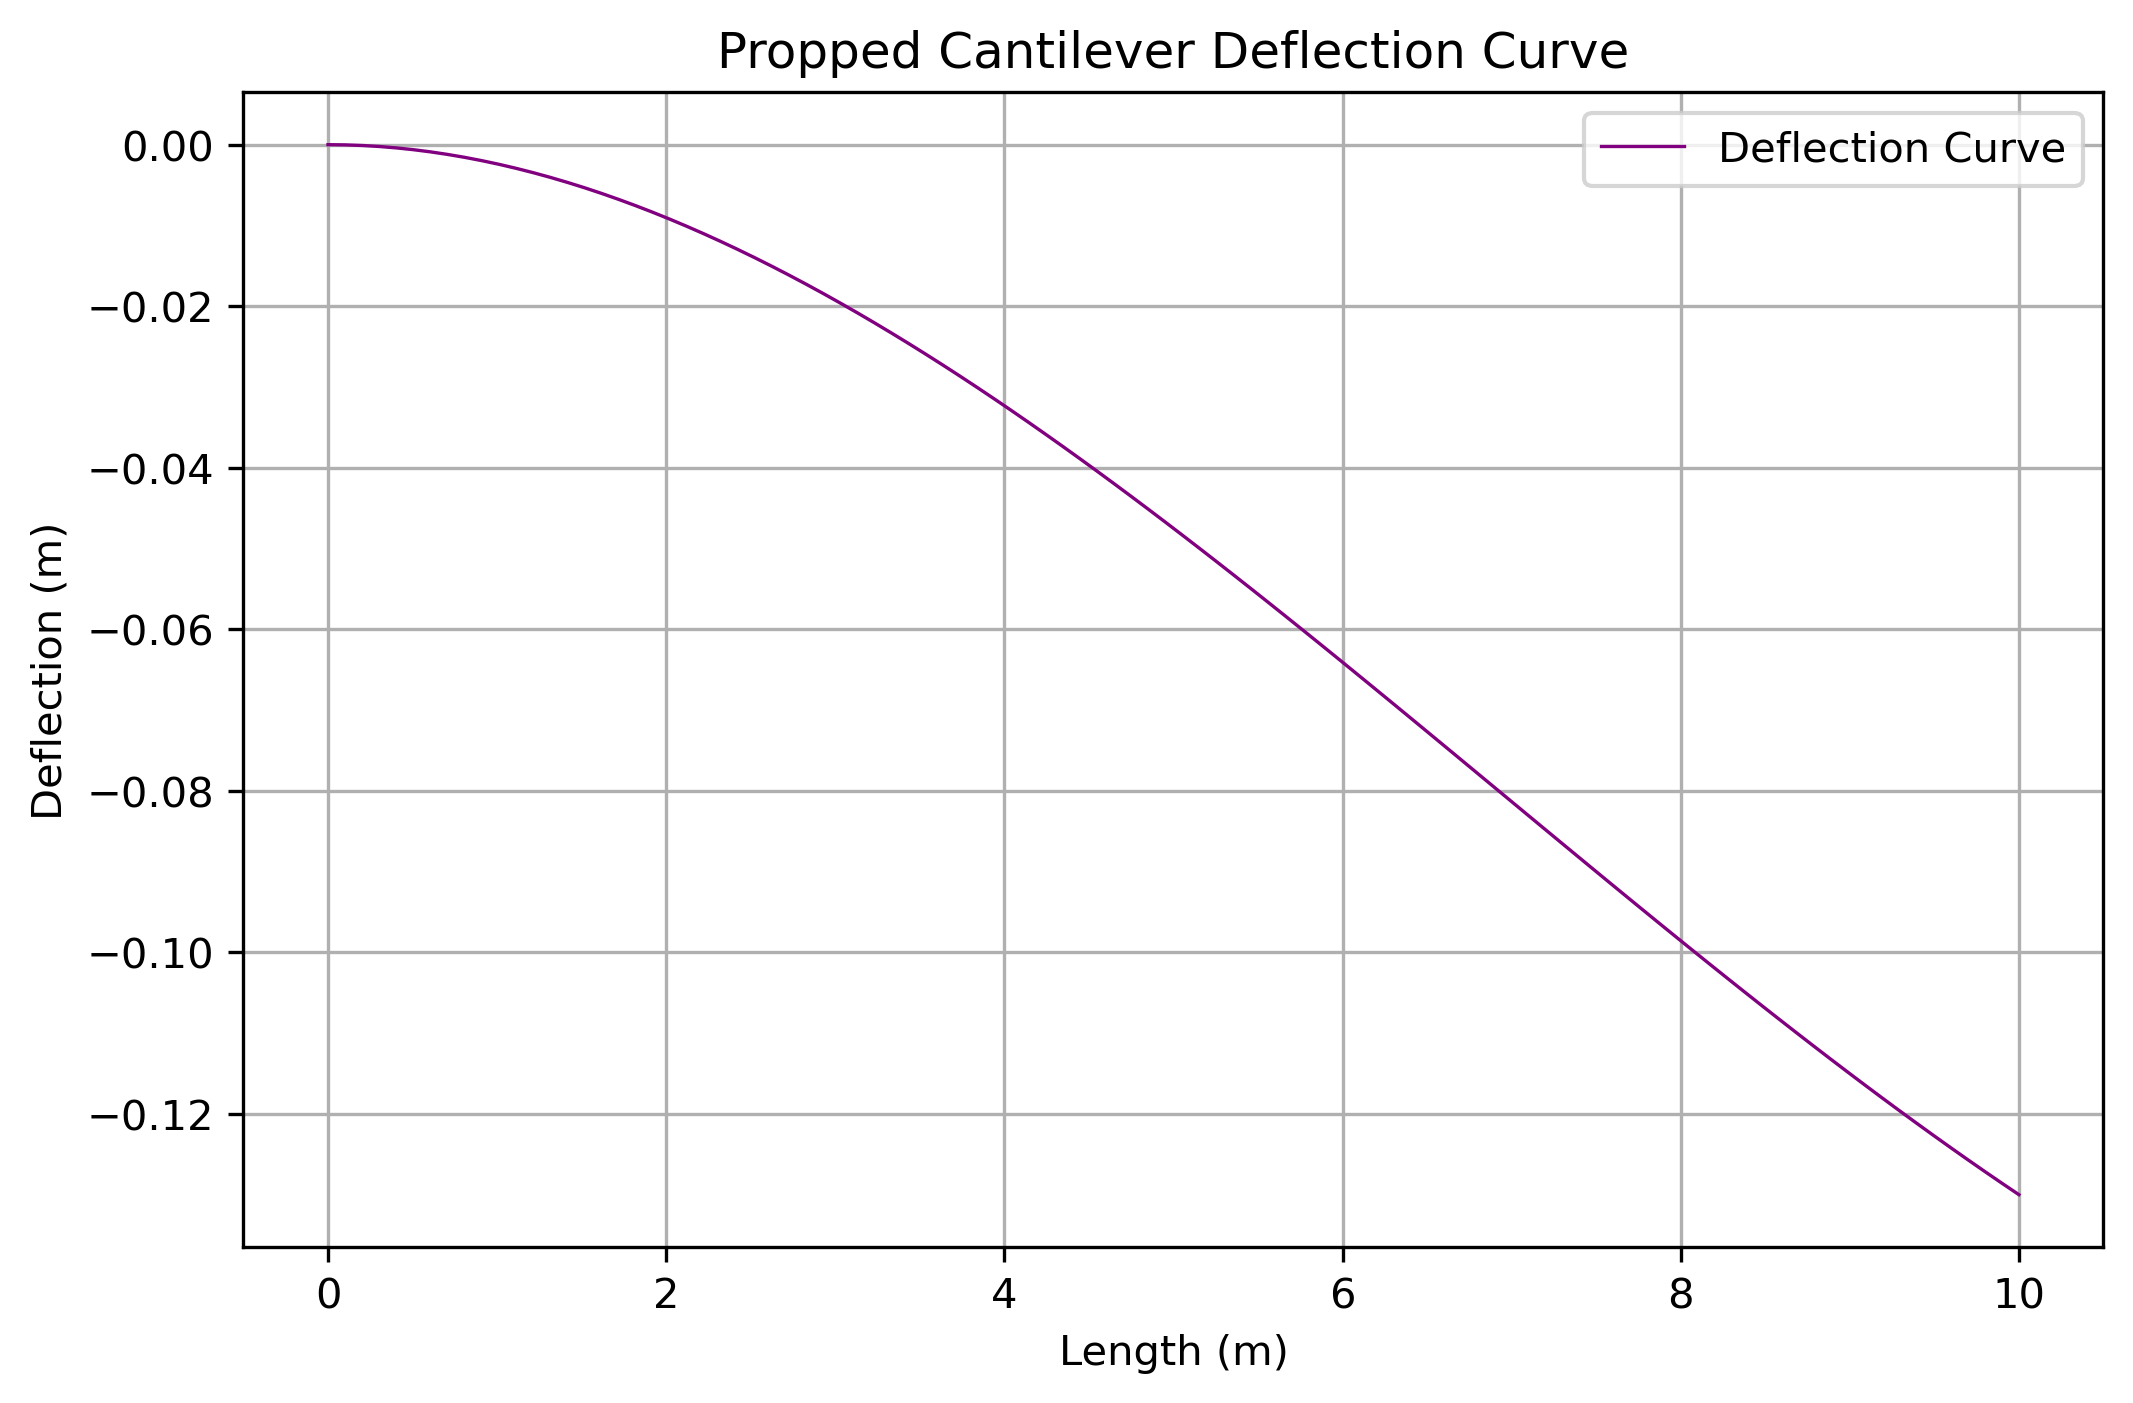
\includegraphics[width=0.95\columnwidth]{figs/cantilever_deflection.png}
    \caption{Propped cantilever and support settlement.}
    \label{fig:ce2q38}
\end{figure}

% ============================================================
% Question 44 — Local extrema of polynomial
% ============================================================

\item
Consider the function given below and pick one or more CORRECT statement(s)
from the following choices.

\begin{equation}
f(x)=x^3-\frac{15}{2}x^2+18x+20
\end{equation}

\hfill (CE2~2025)

\begin{multicols}{2}\begin{enumerate}[label=\alph*)]
    \item \(f(x)\) has a local minimum at \(x=3\).
    \item \(f(x)\) has a local maximum at \(x=3\).
    \item \(f(x)\) has a local minimum at \(x=2\).
    \item \(f(x)\) has a local maximum at \(x=2\).
\end{enumerate}\end{multicols}

\Solution
To determine the local extrema, we differentiate the function.

\begin{equation}
f'(x)=3x^2-15x+18
\end{equation}

Factorizing,

\begin{equation}
f'(x)=3(x^2-5x+6)=3(x-2)(x-3)
\end{equation}

Thus, the critical points are

\begin{equation}
x=2,\qquad x=3
\end{equation}

Now compute the second derivative:

\begin{equation}
f''(x)=6x-15
\end{equation}

At \(x=2\),

\begin{equation}
f''(2)=12-15=-3<0
\end{equation}

Hence, \(f(x)\) has a local maximum at \(x=2\).

At \(x=3\),

\begin{equation}
f''(3)=18-15=3>0
\end{equation}

Hence, \(f(x)\) has a local minimum at \(x=3\).

Therefore, the correct statements are

\begin{equation}
\text{(A) and (D)}
\end{equation}

\begin{figure}[H]
    \centering
    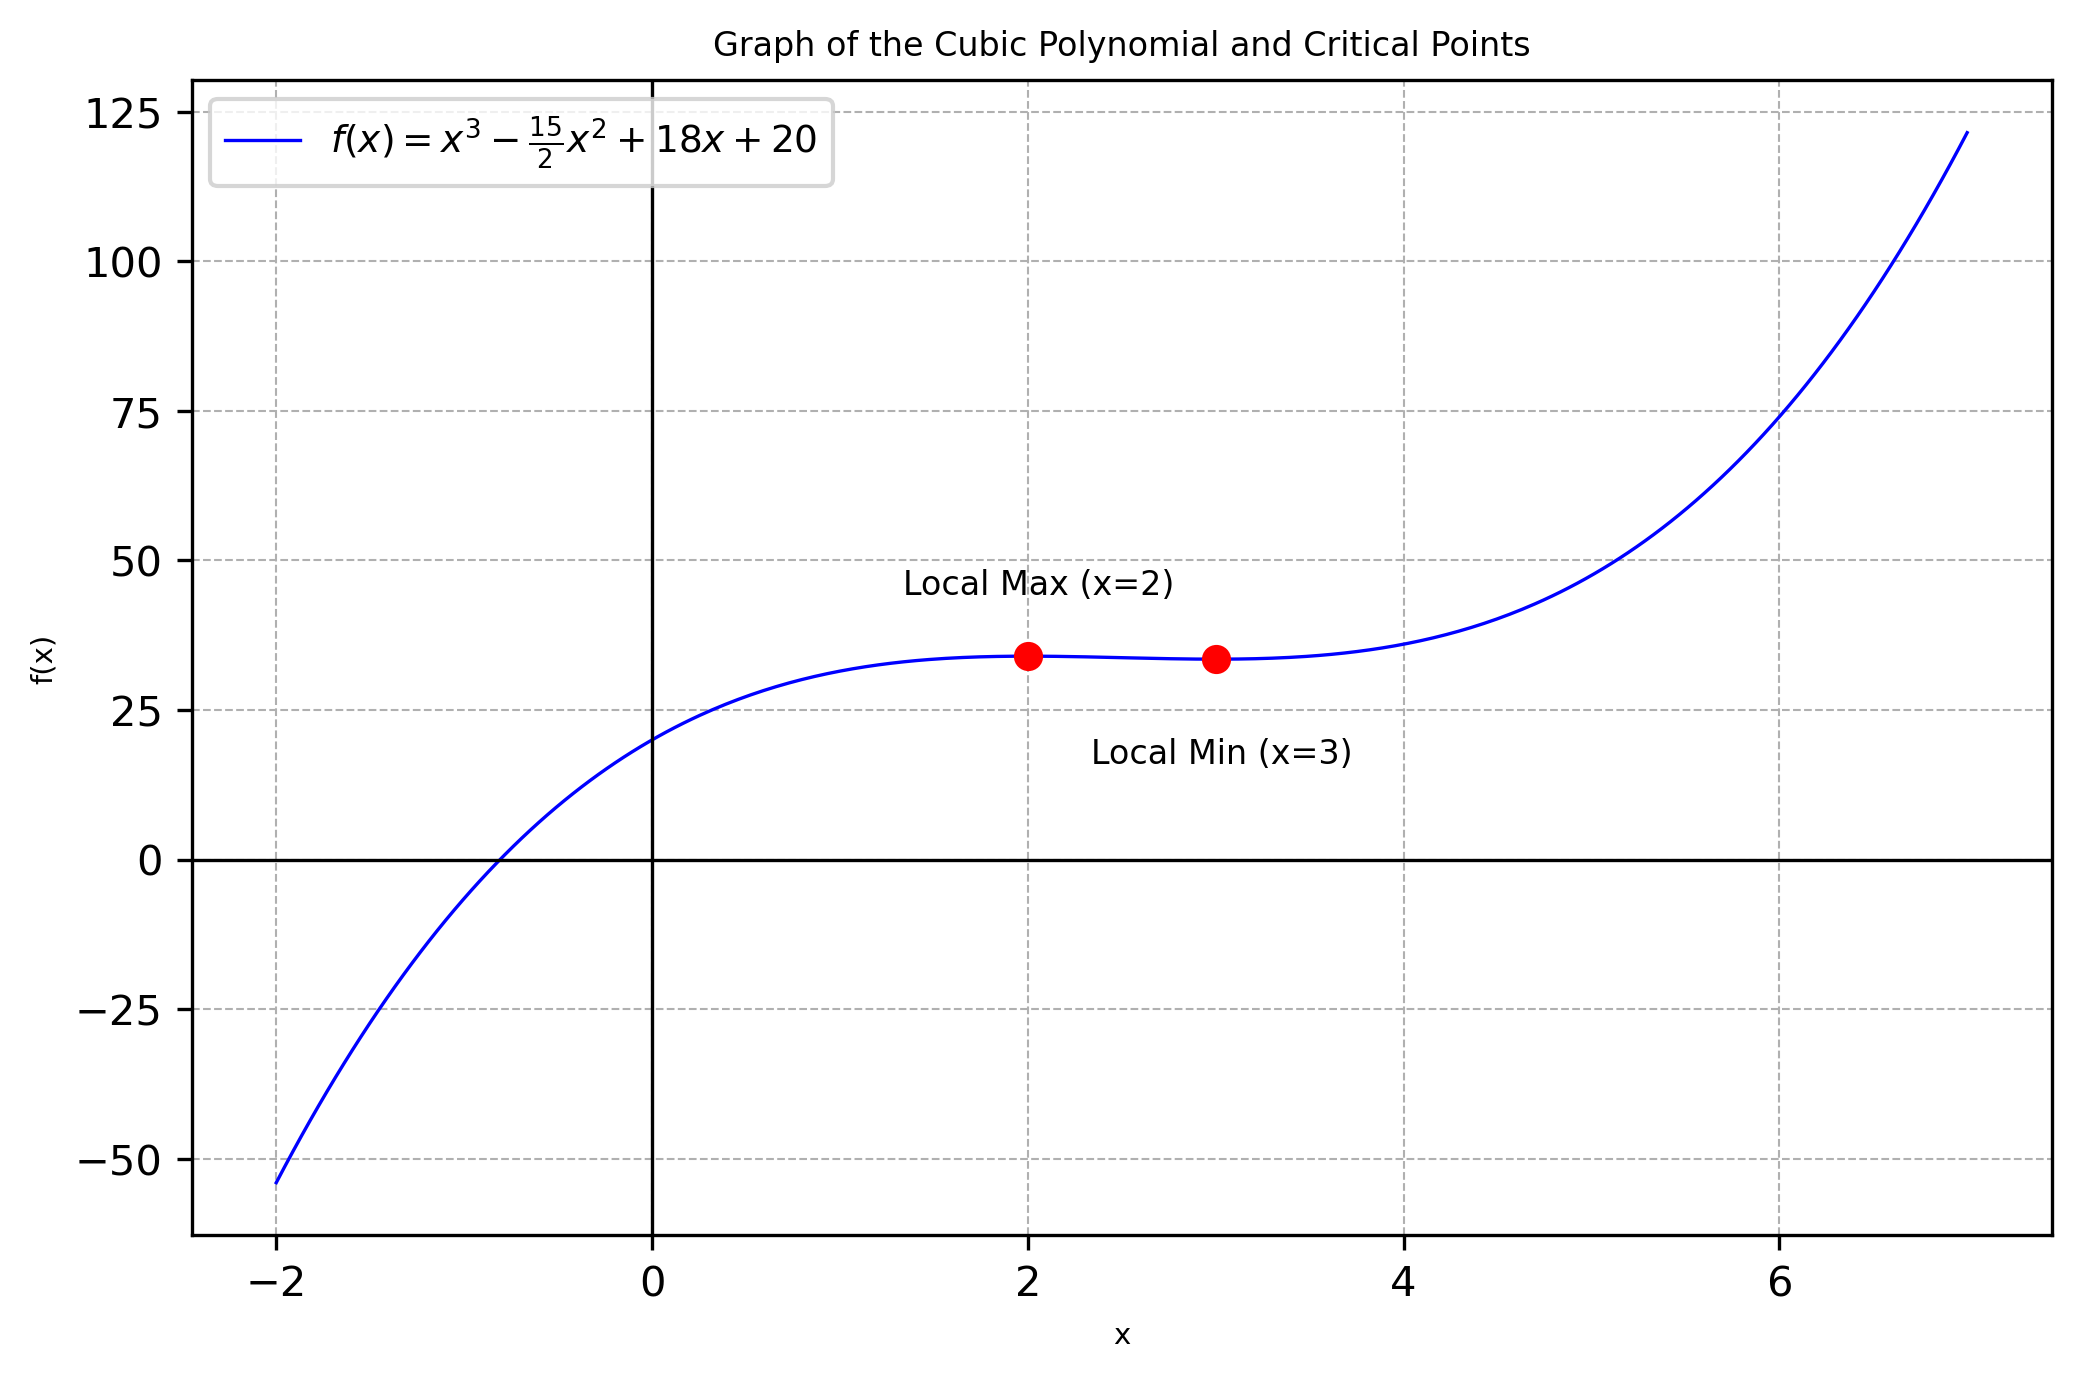
\includegraphics[width=0.86\columnwidth]{figs/cubic.png}
    \caption{Graph of the cubic function in Problem 1.2.13.}
    \label{fig:cubic}
\end{figure}

\CodeRef{codes/ce2q44/ce2q44.py}



\ProblemSpace
% ============================================================
% Question 45 — Eigenvalues of matrix
% ============================================================

\item
Pick the CORRECT eigenvalue(s) of the matrix $\vec{A}$ from the following choices.

\begin{equation}
\vec{A}=
\begin{pmatrix}
6 & 8\\
4 & 2
\end{pmatrix}
\end{equation}

\hfill (CE2~2025)

\begin{multicols}{4}\begin{enumerate}[label=\alph*)]
    \item \(10\)
    \item \(4\)
    \item \(-2\)
    \item \(-10\)
\end{enumerate}\end{multicols}

\Solution
The eigenvalues are obtained from the characteristic equation

\begin{equation}
\det(\vec{A}-\lambda I)=0
\end{equation}

Therefore,

\begin{equation}
\det
\begin{pmatrix}
6-\lambda & 8\\
4 & 2-\lambda
\end{pmatrix}=0
\end{equation}

Expanding,

\begin{equation}
(6-\lambda)(2-\lambda)-32=0
\end{equation}

\begin{equation}
12-8\lambda+\lambda^2-32=0
\end{equation}

\begin{equation}
\lambda^2-8\lambda-20=0
\end{equation}

Factoring,

\begin{equation}
(\lambda-10)(\lambda+2)=0
\end{equation}

Hence, the eigenvalues are

\begin{equation}
\lambda=10,\qquad \lambda=-2
\end{equation}

So, the correct options are

\begin{equation}
\text{(A) and (C)}
\end{equation}

\CodeRef{codes/ce2q45/ce2q45.py}



\ProblemSpace
% ============================================================
% Question 46 — Zero-force members in truss
% ============================================================

\item
In the pin-jointed truss shown in the figure, the members that carry zero force are
identified. Which of the following options is/are zero-force members?

\begin{figure}[H]
    \centering
    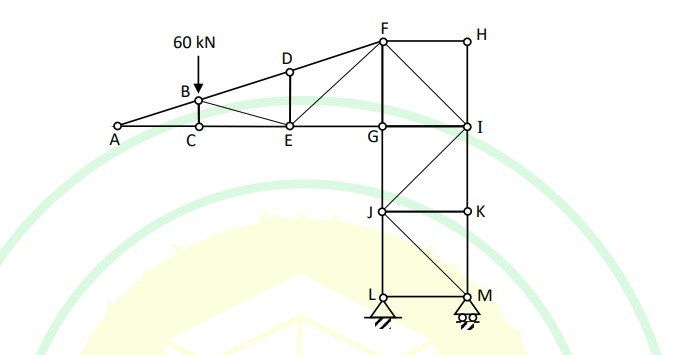
\includegraphics[width=1\columnwidth]{figs/ce2q46.png}
    \label{fig:ce2q46}
\end{figure}

\hfill (CE2~2025)

\begin{multicols}{4}\begin{enumerate}[label=\alph*)]
    \item \(BC\)
    \item \(EG\)
    \item \(FI\)
    \item \(JK\)
\end{enumerate}\end{multicols}

\Solution
We apply the standard zero-force member rules for pin-jointed trusses:

\begin{enumerate}
    \item \textbf{At Joint C:} The bottom chord members $AC$ and $CE$ are collinear, and no external load acts at joint $C$ (the $60\text{ kN}$ load is applied at joint $B$ directly above). Therefore, by the zero-force member rule, member $BC$ carries zero force:
    \begin{align}
    BC &= 0
    \end{align}
    
    \item \textbf{At Joint J:} The horizontal chord members meeting at joint $J$ are collinear, and no external load or support reaction is applied at joint $J$. Hence, member $JK$ carries zero force:
    \begin{align}
    JK &= 0
    \end{align}
\end{enumerate}

Thus, among the choices provided, both $BC$ and $JK$ are zero-force members.

Therefore, the correct options are:

\begin{equation}
\text{(A) and (D)}
\end{equation}

\CodeRef{codes/ce2q46/ce2q46.py}


\ProblemSpace
% ============================================================
% Question 49 — Empirical formula from TOC, COD and TKN
% ============================================================

\item
A compound has a general formula \(C_aH_bO_cN_d\) and molecular weight 187.
A \(935\) mg/l solution of the compound is prepared in distilled deionized water.
The Total Organic Carbon (TOC) is measured as \(360\) mg/l (as C). The Chemical
Oxygen Demand (COD) and the Total Kjeldahl Nitrogen (TKN) are determined as
\(600\) mg/l (as \(O_2\)) and \(140\) mg/l (as N), respectively.

As per the reaction
\begin{equation}
C_aH_bO_cN_d + \left(\frac{4a+b-2c-3d}{4}\right)O_2
\rightarrow aCO_2 + \frac{b-3d}{2}H_2O + dNH_3
\end{equation}

which of the following options is/are CORRECT?

Atomic weights: $C=12$, $H=1$, $O=16$, $N=14$

\begin{table}[H]
\centering
\caption{Given data for the compound.}
\begin{tabular}{@{}lc@{}}
\hline
\textbf{Quantity} & \textbf{Value} \\
\hline
Molecular weight & $187$ \\
Solution concentration & $935$ mg/l \\
TOC & $360$ mg/l as C \\
COD & $600$ mg/l as $O_2$ \\
TKN & $140$ mg/l as N \\
\hline
\end{tabular}
\end{table}

\hfill (CE2~2025)

\begin{multicols}{4}\begin{enumerate}[label=\alph*)]
    \item \(a=6\)
    \item \(b=7\)
    \item \(c=5\)
    \item \(d=3\)
\end{enumerate}\end{multicols}

\Solution
The concentration of the compound is \(935\) mg/l \(=0.935\) g/l. Since the molecular
weight is \(187\), the molar concentration is
\begin{equation}
\frac{0.935}{187}=5\times 10^{-3}\ \text{mol/l}
\end{equation}

From TOC,
\begin{equation}
(5\times 10^{-3})(12a)=360\times 10^{-3}
\end{equation}
\begin{equation}
0.06a=0.36
\quad\Rightarrow\quad
a=6
\end{equation}

From TKN,
\begin{equation}
(5\times 10^{-3})(14d)=140\times 10^{-3}
\end{equation}
\begin{equation}
0.07d=0.14
\quad\Rightarrow\quad
d=2
\end{equation}

Hence, option (D) is false.

Using molecular weight,
\begin{equation}
12a+b+16c+14d=187
\end{equation}
Substituting \(a=6\) and \(d=2\),
\begin{equation}
72+b+16c+28=187
\end{equation}
\begin{equation}
b+16c=87
\end{equation}

From COD data, oxygen consumed is \(600\) mg/l \(=0.6\) g/l. Therefore, oxygen
consumed per mole of compound is
\begin{equation}
\frac{0.6}{5\times 10^{-3}}=120\ \text{g/mol of } O_2
\end{equation}
Hence,
\begin{equation}
\text{moles of }O_2=\frac{120}{32}=3.75
\end{equation}

From the given reaction,
\begin{equation}
\frac{4a+b-2c-3d}{4}=3.75
\end{equation}
Substituting \(a=6\) and \(d=2\),
\begin{equation}
\frac{24+b-2c-6}{4}=3.75
\end{equation}
\begin{equation}
18+b-2c=15
\end{equation}
\begin{equation}
b-2c=-3
\end{equation}

Now write the two equations in matrix form:
\begin{equation}
\myvec{1&16\\1&-2}
\myvec{b\\c}
=
\myvec{87\\-3}.
\end{equation}

Using explicit row reduction,
\begin{equation}
\resizebox{0.95\linewidth}{!}{$
\left[\begin{array}{cc|c}
1&16&87\\
1&-2&-3
\end{array}\right]
\xrightarrow{\;R_2\leftarrow R_2-R_1\;}
\left[\begin{array}{cc|c}
1&16&87\\
0&-18&-90
\end{array}\right]
\xrightarrow{\;R_2\leftarrow-\frac{1}{18}R_2\;}
\left[\begin{array}{cc|c}
1&16&87\\
0&1&5
\end{array}\right]
\xrightarrow{\;R_1\leftarrow R_1-16R_2\;}
\left[\begin{array}{cc|c}
1&0&7\\
0&1&5
\end{array}\right].$}
\end{equation}

Therefore,
\begin{align}
b&=7, & c&=5,\\
a&=6, & d&=2.
\end{align}

Thus,
\begin{equation}
C_aH_bO_cN_d= C_6H_7O_5N_2.
\end{equation}

Therefore, the correct options are (A), (B) and (C).

\CodeRef{codes/ce2q49/ce2q49.py}



\ProblemSpace
% ============================================================
% Question 51 — Standard deviation of discrete random variable
% ============================================================

\item
Consider a discrete random variable \(X\) whose probabilities are given below.
The standard deviation of the random variable is \underline{\hspace{2cm}}
(round off to one decimal place).

\begin{table}[H]
\centering
\caption{Probability distribution of $X$.}
\begin{tabular}{@{}c|cccc@{}}
\hline
$x_i$ & $1$ & $2$ & $4$ & $8$\\ \hline
$P(X=x_i)$ & $0.3$ & $0.1$ & $0.3$ & $0.3$\\
\hline
\end{tabular}
\end{table}

\hfill (CE2~2025)

\Solution
The mean is

\begin{equation}
\mu = E[X] = \sum x_i p_i
\end{equation}

\begin{equation}
\mu = 1(0.3)+2(0.1)+4(0.3)+8(0.3)
\end{equation}

\begin{equation}
\mu = 0.3+0.2+1.2+2.4=4.1
\end{equation}

Now,

\begin{equation}
E[X^2]=1^2(0.3)+2^2(0.1)+4^2(0.3)+8^2(0.3)
\end{equation}

\begin{equation}
E[X^2]=0.3+0.4+4.8+19.2=24.7
\end{equation}

Hence the variance is

\begin{equation}
\sigma^2 = E[X^2]-\mu^2
\end{equation}

\begin{equation}
\sigma^2 = 24.7-(4.1)^2 = 24.7-16.81 = 7.89
\end{equation}

Therefore, the standard deviation is

\begin{equation}
\sigma = \sqrt{7.89}=2.81
\end{equation}

Rounded off to one decimal place,

\begin{equation}
2.8
\end{equation}

\CodeRef{codes/ce2q51/ce2q51.c}



\begin{comment}

\ProblemSpace
% ============================================================
% Question 52 — Beam suspended by three steel rods
% ============================================================

\item
A steel beam supported by three parallel pin-jointed steel rods is shown in the figure.
The moment of inertia of the beam is \(8\times 10^7\) mm\(^4\). Take modulus of elasticity
of steel as \(210\) GPa. The beam is subjected to uniformly distributed load of
\(6.25\) kN/m, including its self-weight.

The axial force (in kN) in the centre rod \(CD\) is \underline{\hspace{2cm}}
(round off to one decimal place).

\hfill (CE2~2025)

\Solution
Let the axial forces in rods \(AB\), \(CD\), and \(EF\) be \(R_B\), \(R_D\), and \(R_F\),
respectively. By symmetry,
\begin{equation}
R_B = R_F
\end{equation}

The total uniformly distributed load on the beam is
\begin{equation}
wL = 6.25\times 4 = 25 \text{ kN}
\end{equation}
Hence, from vertical equilibrium,
\begin{equation}
R_B + R_D + R_F = 25
\end{equation}
or
\begin{equation}
2R_B + R_D = 25
\end{equation}

The rods act as elastic supports. Their stiffness is
\begin{equation}
k=\frac{AE}{L_r}
\end{equation}
where \(L_r=1\) m \(=1000\) mm.

For the side rods \((12\text{ mm diameter})\),
\begin{equation}
A_s=\frac{\pi}{4}(12)^2
\end{equation}
\begin{equation}
k_s=\frac{A_sE}{L_r}
\end{equation}

For the centre rod \((30\text{ mm diameter})\),
\begin{equation}
A_c=\frac{\pi}{4}(30)^2
\end{equation}
\begin{equation}
k_c=\frac{A_cE}{L_r}
\end{equation}

Thus,
\begin{equation}
k_s=\frac{\pi}{4}(12)^2\frac{210\times10^3}{1000}
=23750.4\ \text{N/mm}
\end{equation}
\begin{equation}
k_c=\frac{\pi}{4}(30)^2\frac{210\times10^3}{1000}
=148440.3\ \text{N/mm}
\end{equation}

Let the vertical deflections of the beam at \(B\), \(D\), and \(F\) be \(\delta_B\), \(\delta_D\),
and \(\delta_F\), respectively. Then,
\begin{equation}
\delta_B=\frac{R_B}{k_s},\qquad
\delta_D=\frac{R_D}{k_c},\qquad
\delta_F=\frac{R_F}{k_s}
\end{equation}

Since the system is symmetric,
\begin{equation}
\delta_B=\delta_F,\qquad R_B=R_F
\end{equation}

Now use beam flexibility coefficients for a simply supported beam of span \(4\) m,
with support points at \(x=0,2,4\) m. The deflections at \(B\) and \(D\) due to the UDL
and the point reactions satisfy the compatibility equations:
\begin{equation}
\delta_B = \delta_B^{(w)} - f_{BB}R_B - f_{BD}R_D - f_{BF}R_F
\end{equation}
\begin{equation}
\delta_D = \delta_D^{(w)} - f_{DB}R_B - f_{DD}R_D - f_{DF}R_F
\end{equation}

Using symmetry \((R_B=R_F)\), these reduce to two equations in \(R_B\) and \(R_D\).
Substituting the flexibility coefficients for the beam \((EI = 210\times10^3 \times 8\times10^7
=1.68\times10^{13}\ \text{N\,mm}^2)\), and solving together with
\begin{equation}
2R_B+R_D=25
\end{equation}
gives
\begin{equation}
R_B \approx 4.25\ \text{kN},\qquad R_D \approx 16.5\ \text{kN}
\end{equation}

Therefore, the axial force in the centre rod \(CD\) is
\begin{equation}
16.5
\end{equation}

\CodeRef{codes/ce2q52/ce2q52.py}




\ProblemSpace
% ============================================================
% Question 65 — Interior angle from fore bearings
% ============================================================

\item
If the Fore Bearing of the lines \(AB\) and \(BC\) are \(60^\circ\) and \(122^\circ\),
respectively, then the interior angle \(\angle ABC\) (in degrees) is
\underline{\hspace{2cm}} (round off to the nearest integer).

\hfill (CE2~2025)

\Solution
The fore bearing of line \(AB\) is

\begin{equation}
\text{FB}_{AB}=60^\circ
\end{equation}

Hence the back bearing of line \(BA\) is

\begin{equation}
\text{BB}_{BA}=60^\circ+180^\circ=240^\circ
\end{equation}

The fore bearing of line \(BC\) is

\begin{equation}
\text{FB}_{BC}=122^\circ
\end{equation}

The interior angle at \(B\), that is \(\angle ABC\), is the angle between the directions
\(BA\) and \(BC\). Therefore,

\begin{equation}
\angle ABC = |240^\circ-122^\circ|=118^\circ
\end{equation}

Hence,

\begin{equation}
118^\circ
\end{equation}

\CodeRef{codes/ce2q65/ce2q65.py}


\begin{figure}[H]
    \centering
    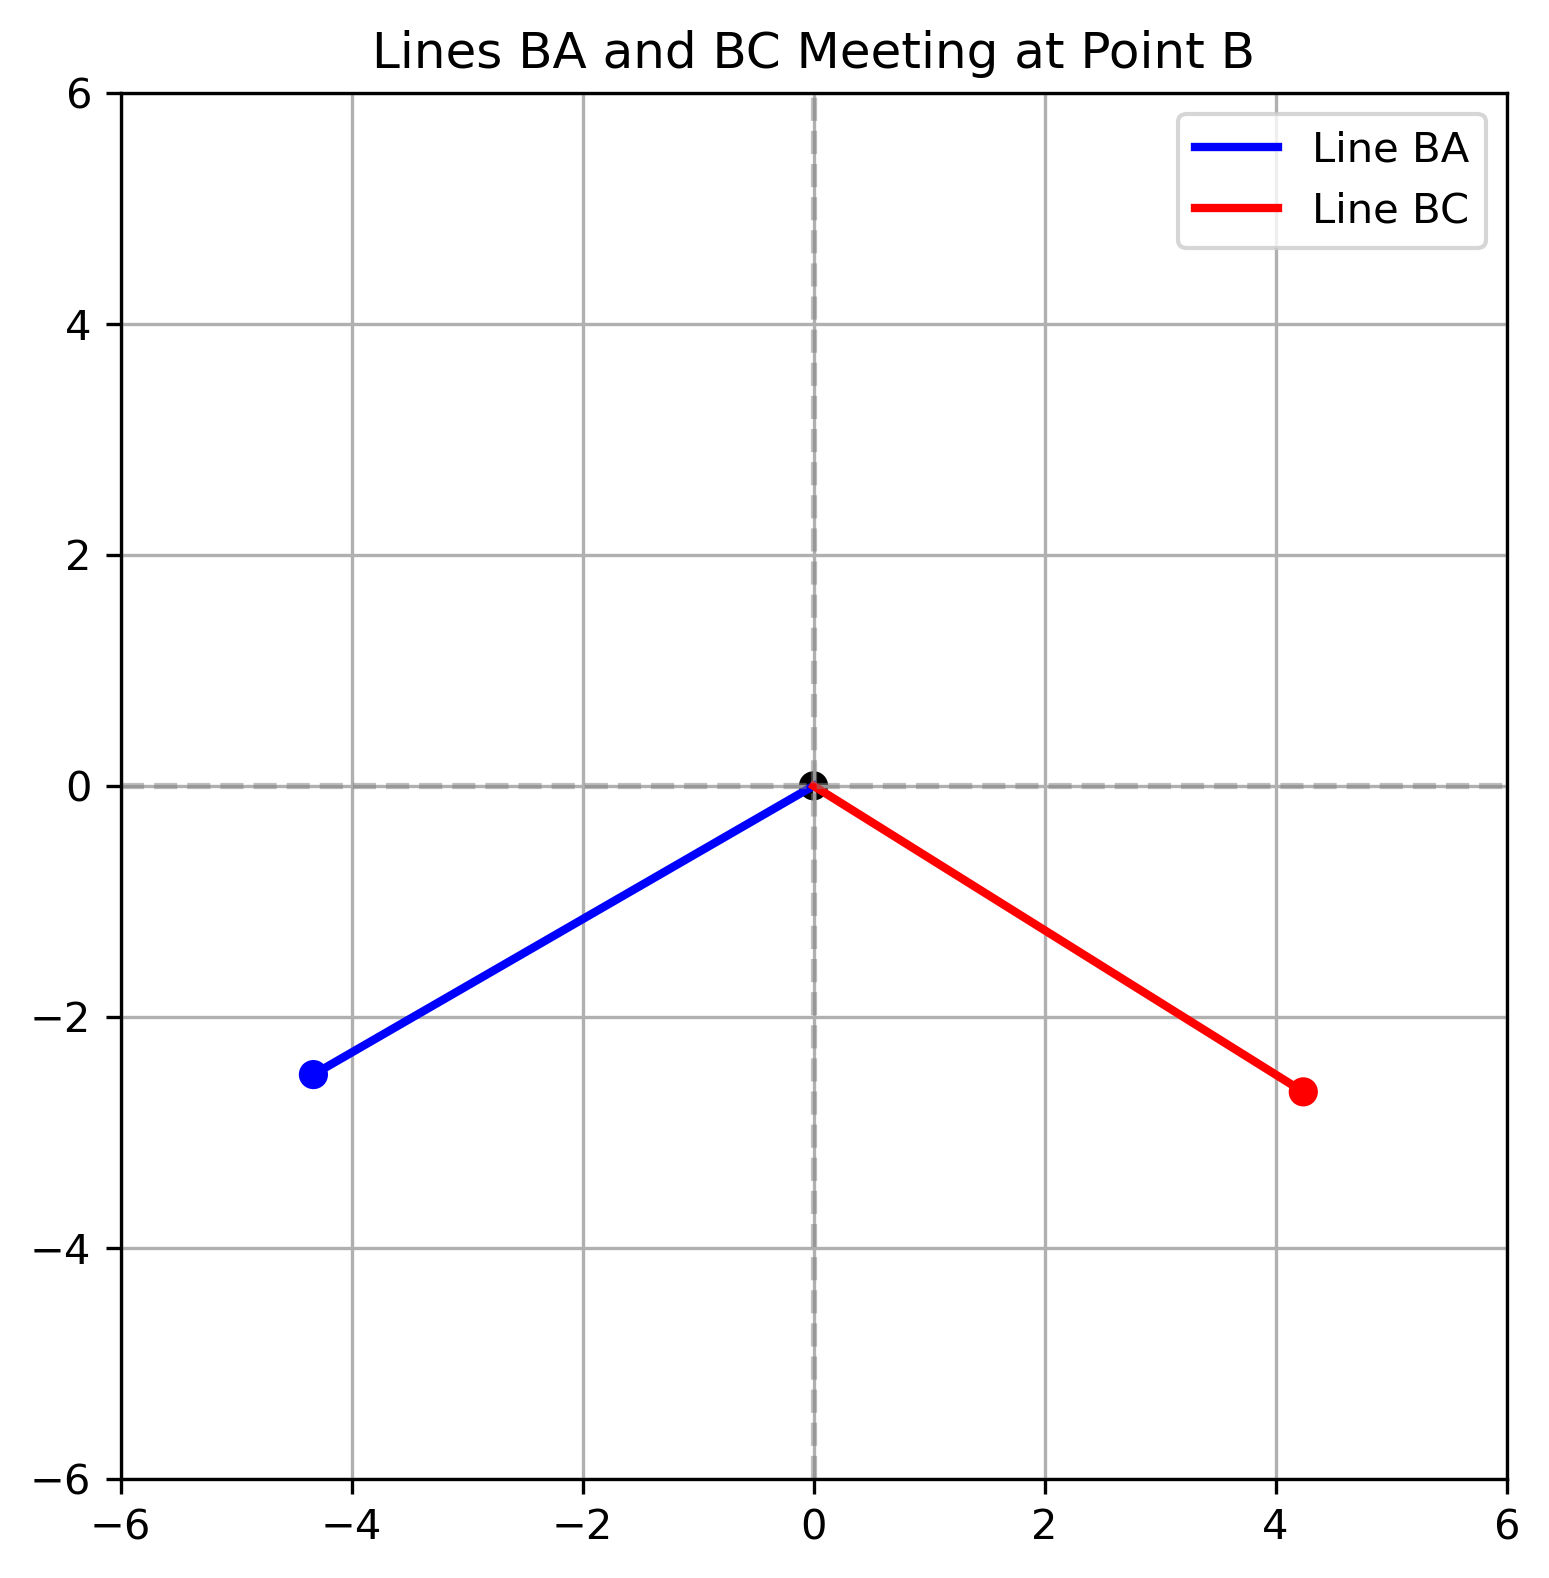
\includegraphics[width=1\columnwidth]{figs/interior_angle.png}
    \label{fig:ce2q65}
\end{figure}




\end{comment}

\end{enumerate}